\documentclass{standalone}
\usepackage{tikz}
\begin{document}
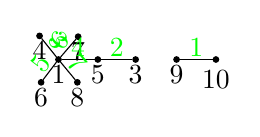
\begin{tikzpicture}[every node/.style={draw, circle, fill=black, minimum size=2pt, inner sep=0pt}]
\node[fill=black, label=below:{\color{black}$6$}] (G1N6) at (4.23,6.16) {};
\node[fill=black, label=below:{\color{black}$1$}] (G1N1) at (4.45,6.45) {};
\node[fill=black, label=below:{\color{black}$5$}] (G1N5) at (4.95,6.45) {};
\node[fill=black, label=below:{\color{black}$3$}] (G1N3) at (5.43,6.45) {};
\node[fill=black, label=below:{\color{black}$7$}] (G1N7) at (4.70,6.74) {};
\node[fill=black, label=below:{\color{black}$8$}] (G1N8) at (4.69,6.16) {};
\node[fill=black, label=below:{\color{black}$4$}] (G1N4) at (4.21,6.75) {};
\node[fill=black, label=below:{\color{black}$9$}] (G1N9) at (5.95,6.45) {};
\node[fill=black, label=below:{\color{black}$10$}] (G1N10) at (6.45,6.45) {};
\draw (G1N1) -- node[midway, sloped, above, draw=none, fill=none] {\textcolor{green}{4}} (G1N5);
\draw (G1N1) -- node[midway, sloped, above, draw=none, fill=none] {\textcolor{green}{5}} (G1N6);
\draw (G1N1) -- node[midway, sloped, above, draw=none, fill=none] {\textcolor{green}{6}} (G1N7);
\draw (G1N1) -- node[midway, sloped, above, draw=none, fill=none] {\textcolor{green}{7}} (G1N8);
\draw (G1N1) -- node[midway, sloped, above, draw=none, fill=none] {\textcolor{green}{3}} (G1N4);
\draw (G1N5) -- node[midway, sloped, above, draw=none, fill=none] {\textcolor{green}{2}} (G1N3);
\draw (G1N9) -- node[midway, sloped, above, draw=none, fill=none] {\textcolor{green}{1}} (G1N10);
\end{tikzpicture}
\end{document}
